\startfirstchapter{Introduction}
\label{chapter:introduction}

The Standard Model (SM) of particle physics stands as one of our most scrutinized and well-tested theories in physics.
Very few discrepancies have been found between the model and reality, within the realm of experimental particle physics.
The discovery of the Higgs boson in July 2012 stands as the most recent example, with the measured quantities thus far matching the Standard Model Higgs boson.
However, it must be the case that the theory is incomplete, as we currently do not know how to incorporate the effects of gravity into the model.
In order to make progress, one can look to the few experiments that provide some level of discrepancy; these could act as a loose string that we can use to unravel the current mysteries of particle physics.

Historically, experimental anomalies have been used as a foundation to construct our understanding of particle physics.
For example, the solar neutrino problem was an anomaly that led to the eventual discovery of neutrino oscillations; the Homestake experiment \cite{Davis:1968cp} in the 1960s would house a large vat of perchloroethylene underground, looking for evidence of neutrino capture via $\nu_e +~^{37}\textrm{Cl} \rightarrow~^{37}\textrm{Ar} + e^-$.
The results compared to theoretical calculations yielded a deficit by a factor of three.
Other experimental efforts were also established to measure the flux of solar neutrinos, such as \sage \cite{Abdurashitov:1999zd}, \gallex \cite{Hampel:1998xg}, \sno \cite{Boger:1999bb}, Kamiokande and Super-Kamiokande \cite{Fukuda:1996sz, Fukuda:2002pe}.
Eventually, the realization was that the Homestake experiment was only sensitive to one of the three neutrino flavours, while \sno was the first experiment able to detect the oscillations put forth in 1968 that would lead on to explain the missing solar neutrinos \cite{Gribov:1968kq}.

Muons have long been a source of mystery within the physics community.
They were discovered in 1936 by Carl Anderson and Seth Neddermyer, who observed the distinct curvature of the muon in a magnetic field, compared to that of electrons and protons. Since then, there have been many questions regarding the properties of this particle.
One of the deeper questions of the Standard Model concerns the number of generations of leptons: Why is it that we observe three generations, the electron, muon, and tau? Within the Standard Model, each generation of lepton differs only by the mass assigned to them.

However, while this can be viewed as an aesthetic problem with the model, at least two experimental efforts have revealed discrepancies between the Standard Model muons and reality.
In particular, the muon's spin magnetic moment $g$ appears to be different at the level of $10^{-8}$ which, although a small number, represents a $3.4\sigma$ discrepancy between experiment and theory \cite{2007PhLB..649..173H}.
It is important to note that many tests have been performed with muons that are consistent with the SM.
The \twist experiment at TRIUMF has provided high precision measurements (a few parts in $10,000$) of distributions of decay products with polarized muons \cite{Bayes:2011zza}.
Universality of the electron and muon has also been tested in pion \cite{Czapek:1993kc}, kaon \cite{Antonelli:2008jg}, and Z-boson decays \cite{Alexander:1991qw}.

Additionally, one can perform experiments on \emph{muonic Hydrogen} ($\mu\textrm{H}$) in which the electron orbiting the proton is replaced with a muon.
For both cases of electronic Hydrogen (H) and $\mu\textrm{H}$, the proton charge radius $r_p$, which will be better defined later in the thesis, can be extracted.
Peculiarly, the two results differ by a significant amount, $\Delta(r_p^2) = (r_p^2)_{\textrm{electrons}} - (r_p^2)_{\textrm{muons}} = 0.06~\textrm{fm}^2$, and stand at a $7\sigma$ discrepancy from zero \cite{Carlson:2015jba}.
Regardless of whether H or $\mu\textrm{H}$ is used, the extraction of the proton charge radius should remain unchanged.
This leads to an exciting avenue to search for new physics, and may give some hints to a new physics role for the muon in such a system.

If new physics has the potential to solve some of these problems, then we must know where to look for the new physics.
We will take $\hslash = c = 1$ in this thesis.
Since we have that $G_F \ll \Delta(r_p^2)$, this provides a good indication that, to explain the proton radius discrepancy, we should look for a carrier of a new gauge or Yukawa force much lighter than the electroweak scale.
A light new mediator may be able to solve these issues, such as the dark photon.
It is the goal of this thesis to study the sensitivity limits of detection of such a new light mediator.
In our case we consider a scalar, $\phi$, which violates lepton universality by coupling to leptons proportionally to their mass, very similarly to the SM Higgs boson.
This can have implications for a whole range of experiments, especially at the intensity frontier where precision physics measurements are possible.
A schematic of the landscape is shown in Fig.\ \ref{fig:frontiers}.

\begin{figure}[h]
    \centering
    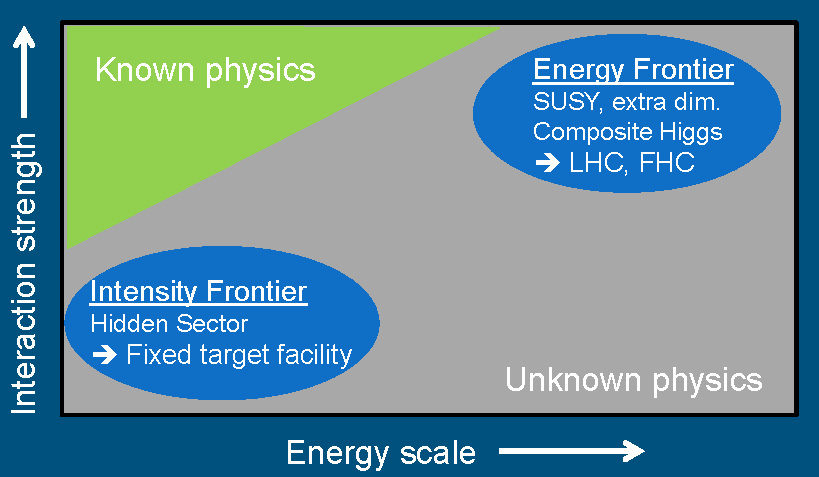
\includegraphics[width = 0.8\textwidth]{Figures/misc/frontiers}
    \caption[Schematic of the frontiers available to experimental particle physics.]{Schematic of the frontiers available to experimental particle physics from \cite{Alekhin:2015byh}. The SM lives in the upper left corner. In order to access heavy physics, such as the top or the Higgs, one must turn to the energy frontier with high energy colliders such as the LHC. Lightly coupled new physics is easier to access where there are many collisions or decays in a short period of time, provided that the energies required to produce the new physics are not large.}
    \label{fig:frontiers}
\end{figure}

The experiment \mueee will have $\order(10^{16})$ total muon decays, so we must investigate how the new force carrying particle interacts with the muon decay signature studied there.
Similarly, the experiments NA48/2 and NA62 study $\order(10^{11})$ kaon decays, and we can use this to place sensitivity limits on the strength of the coupling of the new particle.
Finally, asymmetric $e^+ e^-$ colliders with their associated detectors, like \babar, \belle, and \belletwo, can examine higher energy ranges up to $10.58~\textrm{GeV}$, where the tau lepton becomes kinematically accessible and would strongly couple to our new particle.
Combining these regimes yields sensitivity over a wide range of masses, from $10~\textrm{MeV}$ all the way up to $3.5~\textrm{GeV}$.
The signal processes we will be investigating are the following:

\begin{enumerate}
\item $\mu^+ \rightarrow e^+ \nu_e \bar{\nu_\mu} \phi,~\phi \rightarrow e^+ e^-$
\item $K^+ \rightarrow \mu^+ \nu_\mu \phi,~\phi \rightarrow \ell^+ \ell^-$
\item $e^+ e^- \rightarrow \tau^+ \tau^- \phi,~\phi \rightarrow \ell^+ \ell^-$
\end{enumerate}

\noindent The signature we will be looking for is a spectrally peaked feature where the invariant pair mass can reconstruct the mass of the scalar, $m_{\ell\ell} = m_\phi$.

This thesis contains six core components.
The first of these is this short introduction to the problem and motivation.
Here we provide a small summary of the contents of each chapter.

\textbf{Chapter 2} discusses the physical motivations for this project briefly.
The main focus is on the apparent anomalies that lie within the Standard Model with emphasis on the muon and lepton flavour violation.
Here we will discuss the proton radius problem and the $(g-2)_\mu$ discrepancy.
This chapter will stand as the summary of the experimental hints that motivate us to pursue this project.
From this, we will see that a candidate for solving these problems is a new scalar force, that so far has received less attention in the literature compared to that of a vector mediator.
Later, we will include the restrictions from $(g-2)_\mu$ in our final results of the scalar.
This candidate particle will then be the focus for the rest of the thesis, and the limits on the sensitivity of detection will be the final result.

\textbf{Chapter 3} will examine each experiment in enough detail to place sensible limits on the scalar particle, or derive sensitivity to it for future experiments.
These experiments will span the mass range of a few $\textrm{MeV}$ up to $10~\textrm{GeV}$.
To do this, three classes of experiments will be examined: muon decay, kaon decay, and $e^+ e^-$ collisions.
Muon decay will be studied in the context of the upcoming \mueee experiment, which provides a large number of muon decays to work with.
Kaon decay at the finished experiment NA48/2, and the upcoming NA62 experiment, will provide access to mediator masses above the muon mass.
Finally, $e^+ e^-$ collisions at a centre of mass energy of $10.58~\textrm{GeV}$, as analyzed by the B-factories \babar, \belle, and \belletwo, will provide the greatest coverage of masses, as well as access to the heaviest leptons.

\textbf{Chapter 4} provides the prescription of tools that we use and the analytical methods in which we extract our limits.
The tools include the Monte Carlo generator \madgraph and other utility tools to interface with the generator.
These are used to generate large numbers of signal and background events, in order to study the sensitivity to our model, as finding an analytic expression for some of these decay rates and cross sections can be difficult.
Our sensitivity extraction procedure is also covered here, where we precisely define what we claim an experiment's upper-limit sensitivity is.

\textbf{Chapter 5} contains the results of this work, which are the existing and potential constraints on scalar coupling strength, in the experiments listed above.
Each process analyzed is documented here in detail and the resulting sensitivity is given.
This includes an explicit detailing of the backgrounds that can affect our overall sensitivity, as well as how we bin our data, generated or otherwise.

\textbf{Chapter 6} will conclude the thesis, with a summary of the work completed and results.
There will also be some brief comments on future, related work.
